%%%%%%%%%%%%%%%%%%%%%%%%%%%%%%%%%%%%%%%%%
% Beamer Presentation
% LaTeX Template
% Version 1.0 (10/11/12)
%
% This template has been downloaded from:
% http://www.LaTeXTemplates.com
%
% License:
% CC BY-NC-SA 3.0 (http://creativecommons.org/licenses/by-nc-sa/3.0/)
%
%%%%%%%%%%%%%%%%%%%%%%%%%%%%%%%%%%%%%%%%%

%----------------------------------------------------------------------------------------
%	PACKAGES AND THEMES
%----------------------------------------------------------------------------------------

\documentclass{beamer}

\mode<presentation> {
\usetheme{Madrid}
}

\usepackage{graphicx} % Allows including images
\usepackage{booktabs} % Allows the use of \toprule, \midrule and \bottomrule in tables

%----------------------------------------------------------------------------------------
%	TITLE PAGE
%----------------------------------------------------------------------------------------

\title[Computer Security]{Buffer Overflow Attack} % The short title appears at the bottom of every slide, the full title is only on the title page

\author{Abijith K P \\\ Bosco Frank Paul \\\ Krishna Pingal \\\ K S Kurian} % Your name
\institute[] % Your institution as it will appear on the bottom of every slide, may be shorthand to save space
{
%National Institute of Technology, Calicut \\ % Your institution for the title page
%\medskip
\textit{} % Your email address
}
\date{\today} % Date, can be changed to a custom date

\begin{document}

\begin{frame}
\titlepage % Print the title page as the first slide
\end{frame}

\begin{frame}
\frametitle{Overview} % Table of contents slide, comment this block out to remove it
\tableofcontents % Throughout your presentation, if you choose to use \section{} and \subsection{} commands, these will automatically be printed on this slide as an overview of your presentation
\end{frame}

%----------------------------------------------------------------------------------------
%	PRESENTATION SLIDES
%----------------------------------------------------------------------------------------

%------------------------------------------------
\section{What is Buffer Overflow}
\begin{frame}
\frametitle{What is Buffer Overflow}
\begin{itemize}
\item \visible<1->{While writting data to buffer} \\\
\item \visible<2->{Overruns the buffer's boundary} \\\
\item \visible<3->{Overwrites adjacent memory.} \\\
\end{itemize}
\end{frame}

\begin{frame}
 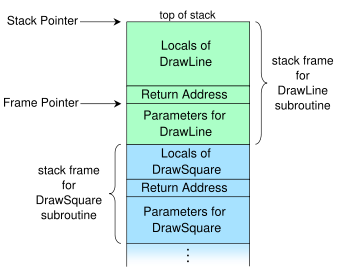
\includegraphics[]{callStack.png}
\end{frame}

\section{What we are doing}
\begin{frame}
 \frametitle {What we are doing}
 \begin{itemize}
  \item \visible<1->{Overwriting the return address in a stack frame: Once the function returns, execution will resume at the return address as specified by the attacker, usually a user input filled buffer} \\\
  \item \visible<2->{Overwriting a local variable that is near the buffer in memory on the stack to change the behavior of the program which may benefit the attacker}
 \end{itemize}
\end{frame}

\section{Mark distribution}
\begin{frame}
 \frametitle {Mark distribution}
 \begin{itemize}
  \item \visible<1-> {Final Presentation: 30 marks}
  \item \visible<2-> {Team completing the task: 70 marks}
  \item \visible<3-> {Hands on demonstration: 100 marks}
  \item \visible<4-> {Total: 200 marks} \\\
 \end{itemize}
\end{frame}


\begin{frame}
\Huge{\centerline{Thank You}}
\end{frame}

%----------------------------------------------------------------------------------------

\end{document} 